% CS6140 Homework Assignment Template
% Computer Science
% Northeastern University
% Boston, MA 02115

% Do not manipulate any of the settings
\documentclass[twoside]{article}
\usepackage{graphicx}
% \graphicspath{ {./images/} }
\usepackage{epsfig}
\usepackage{natbib}
\usepackage{units}
\usepackage{amssymb}
\usepackage{amsmath}
\usepackage{babel}


\setlength{\oddsidemargin}{0 in}
\setlength{\evensidemargin}{0 in}
\setlength{\topmargin}{-0.6 in}
\setlength{\textwidth}{6.5 in}
\setlength{\textheight}{8.5 in}
\setlength{\headsep}{0.75 in}
\setlength{\parindent}{0 in}
\setlength{\parskip}{0.1 in}

\newcommand{\lecture}[3]{
   \pagestyle{myheadings}
   \thispagestyle{plain}
   \newpage
   \setcounter{page}{1}
   \noindent
   \begin{center}
   \framebox{
      \vbox{\vspace{2mm}
    \hbox to 6.28in { {\bf CS6140: Machine Learning\hfill} }
       \vspace{6mm}
       \hbox to 6.28in { {\Large \hfill #1  \hfill} }
       \vspace{6mm}
       \hbox to 6.28in { {\it Assigned: #2 \hfill Due: #3} }
      \vspace{2mm}}
   }
   \end{center}
   \markboth{#1}{#1}
   \vspace*{4mm}
}

\begin{document}

% to have alphanumeric enumeration (Hasan's command)
\renewcommand{\labelenumi}{\alph{enumi})}

\lecture{Homework Assignment \# 2}{02/05/2020}{02/18/2020, 11:59pm, through Blackboard}

\begin{center}
Three problems, 95 points in total. Good luck!\\
Prof. Predrag Radivojac, Northeastern University
\end{center}


\textbf{Name: Seyed Ali Sadat Akhavani}

\textbf{Email: sadatakhavani@husky.neu.edu}

%%
%% Problem
%%

\textbf{Problem 1.} (25 points) Naive Bayes classifier. Consider a binary classification problem where there are only four data points in the training set. That is $\mathcal{D}=\left\{ (-1,-1,-),(-1,+1,+),(+1,-1,+),(+1,+1,-)\right\} $, where each tuple $(x_{1},x_{2},y)$ represents a training example with input vector $(x_{1},x_{2})$ and class label $y$.

\begin{enumerate}
\item (10 points) Construct a naive Bayes classifier for this problem and evaluate its accuracy on the training set. Consider ``accuracy'' to be the fraction of correct predictions.

\textbf{Solution:}

I: We should choose the max between these two:
\[
P(Y=+|(-1,-1)) = 1/2 * 1/2 * 1/2 = 1/8
\]
\[
P(Y=-|(-1,-1)) = 1/2 * 1/2 * 1/2 = 1/8
\]
So the result is: +

II: We should choose the max between these two:
\[
P(Y=+|(-1,+1)) = 1/2 * 1/2 * 1/2 = 1/8
\]
\[
P(Y=-|(-1,+1)) = 1/2 * 1/2 * 1/2 = 1/8
\]
So the result is: +

III: We should choose the max between these two:
\[
P(Y=+|(+1,-1)) = 1/2 * 1/2 * 1/2 = 1/8
\]
\[
P(Y=-|(+1,-1)) = 1/2 * 1/2 * 1/2 = 1/8
\]
So the result is: +

IV: We should choose the max between these two:
\[
P(Y=+|(+1,+1)) = 1/2 * 1/2 * 1/2 = 1/8
\]
\[
P(Y=-|(+1,+1)) = 1/2 * 1/2 * 1/2 = 1/8
\]
So the result is: +

We will now calculate the accuracy. The formula had two correct results.
\[
accuracy  = 2 / 4 = 1/2
\]

\item (10 points) Transform the input space into a six-dimensional space $(+1, x_{1}, x_{2}, x_{1}x_{2}, x_{1}^{2}, x_{2}^{2})$ and repeat the previous step.

\textbf{Solution:}

So the new dataset is this:

$D = \{
(+1,-1,-1,+1,+1,+1,-),
(+1,-1,+1,-1,+1,+1,+),
$

$
(+1,+1,-1,-1,+1,+1,+),
(+1,+1,+1,+1,+1,+1,-)
\}
$

I: We should choose the max between these two:
\[
P(Y=+|(+1,-1,-1,+1,+1,+1)) = 2/2 * 1/2 * 1/2 * 0/2 = 0
\]
\[
P(Y=-|(+1,-1,-1,+1,+1,+1)) = 2/2*1/2*1/2*2/2*2/2*2/2 *1/2 = 1/8
\]
So the result is: -

II: We should choose the max between these two:
\[
P(Y=+|(+1,-1,+1,-1,+1,+1)) = 2/2*1/2*1/2*2/2*2/2*2/2 *1/2 = 1/8
\]
\[
P(Y=-|(+1,-1,+1,-1,+1,+1)) = 2/2 * 1/2 * 1/2 * 0/2 = 0
\]
So the result is: +

III: We should choose the max between these two:
\[
P(Y=+|(+1,+1,-1,-1,+1,+1)) = 2/2*1/2*1/2*2/2*2/2*2/2 *1/2 = 1/8
\]
\[
P(Y=-|(+1,+1,-1,-1,+1,+1)) = 2/2 * 1/2 * 1/2 * 0/2 = 0
\]
So the result is: +

IV: We should choose the max between these two:
\[
P(Y=+|(+1,+1,+1,+1,+1,+1)) = 2/2 * 1/2 * 1/2 * 0/2 = 0
\]
\[
P(Y=-|(+1,+1,+1,+1,+1,+1)) = 2/2*1/2*1/2*2/2*2/2*2/2 *1/2 = 1/8
\]
So the result is: -

We will now calculate the accuracy. The formula had four correct results.
\[
accuracy  = 4 / 4 = 1
\]

\item (5 points) Repeat the previous step when the data set accidentally includes the seventh feature, set to $-x_{1}x_{2}$. What is the impact of adding this dependent feature on the classification model?

\textbf{Solution:}

So the new dataset is this:

$D = \{
(+1,-1,-1,+1,+1,+1,-1,-),
(+1,-1,+1,-1,+1,+1,+1,+),
$

$
(+1,+1,-1,-1,+1,+1,+1,+),
(+1,+1,+1,+1,+1,+1,-1,-)
\}
$


I: We should choose the max between these two:
\[
P(Y=+|(+1,-1,-1,+1,+1,+1,-1)) = 2/2 * 1/2 * 1/2 * 0/2 = 0
\]
\[
P(Y=-|(+1,-1,-1,+1,+1,+1,-1)) = 2/2*1/2*1/2*2/2*2/2*2/2 * 0 *1/2 = 0
\]
So the result is: +

II: We should choose the max between these two:
\[
P(Y=+|(+1,-1,+1,-1,+1,+1,+1)) = 2/2*1/2*1/2*2/2*2/2*2/2*0 *1/2 = 0
\]
\[
P(Y=-|(+1,-1,+1,-1,+1,+1,+1)) = 2/2 * 1/2 * 1/2 * 0/2 = 0
\]
So the result is: +

III: We should choose the max between these two:
\[
P(Y=+|(+1,+1,-1,-1,+1,+1,+1)) = 2/2*1/2*1/2*2/2*2/2*2/2*0 *1/2 = 0
\]
\[
P(Y=-|(+1,+1,-1,-1,+1,+1,+1)) = 2/2 * 1/2 * 1/2 * 0/2 = 0
\]
So the result is: +

IV: We should choose the max between these two:
\[
P(Y=+|(+1,+1,+1,+1,+1,+1,-1)) = 2/2 * 1/2 * 1/2 * 0/2 = 0
\]
\[
P(Y=-|(+1,+1,+1,+1,+1,+1,-1)) = 2/2*1/2*1/2*2/2*2/2*2/2*0 *1/2 = 0
\]
So the result is: +


We will now calculate the accuracy. The formula had two correct results. Adding this feature made our formula to generate wrong results for some inputs. It makes all the probabilities equal to zero so all of the predictions are now leading to + for the result.
\[
accuracy  = 2 / 4 = 1/2
\]

\end{enumerate}

%%
%% Problem
%%

\textbf{Problem 2.} (25 points) Consider a binary classification problem in which we want to determine the optimal decision surface. A point $\mathbf{x}$ is on the decision surface if $P(Y=1|\mathbf{x})=P(Y=0|\mathbf{x})$.

\begin{enumerate}
\item (10 points) Find the optimal decision surface assuming that each class-conditional distribution is defined as a two-dimensional Gaussian distribution:
\[
p(\mathbf{x}|Y=i)=\frac{1}{(2\pi)^{\nicefrac{d}{2}} |\mathbf{\Sigma}_{i}|^{\nicefrac{1}{2}}}\cdot e^{-\frac{1}{2}(\mathbf{x}-\mathbf{m}_{i})^{T}\mathbf{\Sigma}_{i}^{-1}(\mathbf{x}-\mathbf{m}_{i})}
\]
where $i \in \left\{ 0, 1\right\}$, $\mathbf{m}_{0}=(1,2)$, $\mathbf{m}_{1}=(6,3)$, $\mathbf{\Sigma}_{0}=\mathbf{\Sigma}_{1}=\mathbf{I}_2$, $P(Y=0)=P(Y=1)=\nicefrac{1}{2}$, $\mathbf{I}_d$ is the $d$-dimensional identity matrix, and $|\mathbf{\Sigma}_{i}|$ is the determinant of $\mathbf{\Sigma}_{i}$.


\textbf{Solution:}

We know that d=2. So x would be like this:
$\begin{bmatrix}
x0\\
x1
\end{bmatrix}$
\[
p(Y=1|x) = p(Y=0|x) \xrightarrow{} p(x|Y=1)*p(Y=1) = p(x|Y=0)*p(Y=0)
\]
\[
1/2*\frac{1}{(2\pi)^1|\Sigma_0|^{1/2}}.e^{-1/2(x-m_0)^T\Sigma_0^-1(x-m_0)} = 
1/2*\frac{1}{(2\pi)^1|\Sigma_1|^{1/2}}.e^{-1/2(x-m_1)^T\Sigma_1^-1(x-m_1)}
\]
\[
e^{-1/2(x-m_1)^T\Sigma_0^-1(x-m_1)} = e^{-1/2(x-m_1)^T\Sigma_1^-1(x-m_1)}
\]
\[
-1/2*(x-(1,2))^T.I_2^{-1}.(x-(1,2)) = -1/2*(x-(6,3))^T.I_2^{-1}.(x-(6,3))
\]
\[
\begin{bmatrix}
x_0 - 1 & x_1 - 2\\
\end{bmatrix}
* I_2 *
\begin{bmatrix}
x_0 - 1\\
x_1 - 2
\end{bmatrix}
=
\begin{bmatrix}
x_0 - 6 & x_1 - 3\\
\end{bmatrix}
* I_2 *
\begin{bmatrix}
x_0 - 6\\
x_1 - 3
\end{bmatrix}
\]
\[
(x_0 - 1)^2 + (x_1 - 2)^2 = (x_0 - 6)^2 + (x_1 - 3)^2
\]
So this will be the final result:
\[
x_1 = -5x_0 + 20
\]


\item (5 points) Generalize the solution from part (a) using $\mathbf{m}_{0}=(m_{01}, m_{02})$, $\mathbf{m}_{1}=(m_{11}, m_{12})$, $\mathbf{\Sigma}_{0}=\mathbf{\Sigma}_{1}=\sigma^2 \mathbf{I}_2$ and $P(Y=0)\neq P(Y=1)$.


\textbf{Solution:}

\[
p_{y_0}.\frac{1}{(2\pi)^1(\sigma^2)^{1/2}}.e^{-1/2(x-m_{01})^T\Sigma_0^-1(x-m_{02})} = 
p_{y_1}.\frac{1}{(2\pi)^1(\sigma^2)^{1/2}}.e^{-1/2(x-m_{11})^T\Sigma_1^-1(x-m_{12})}
\]
\[
p_{y_0}.e^{-1/2(x-m_{01})^T\Sigma_0^-1(x-m_{02})} = p_{y_1}.e^{-1/2(x-m_{11})^T\Sigma_1^-1(x-m_{12})}
\]
\[
\ln{p_{y_0}} -\frac{1}{2}.\sigma^2.(x-(m_{01},m_{02}))^T.I_2^{-1}.(x-(m_{01},m_{02})) = \ln{p_{y_1}} -\frac{1}{2}.\sigma^2.(x-(m_{11},m_{02}))^T.I_2^{-1}.(x-(m_{11},m_{12}))
\]
\[
(-\frac{2}{\sigma^2}.\ln{p_{y_0}}) + (
\begin{bmatrix}
x_0 - m_{01} & x_1 - m_{02}\\
\end{bmatrix}
* I_2 *
\begin{bmatrix}
x_0 - m_{01}\\
x_1 - m_{02}
\end{bmatrix}
)
=
(-\frac{2}{\sigma^2}.\ln{p_{y_1}}) + (
\begin{bmatrix}
x_0 - m_{11} & x_1 - m_{12}\\
\end{bmatrix}
* I_2 *
\begin{bmatrix}
x_0 - m_{11}\\
x_1 - m_{12}
\end{bmatrix}
)
\]

% m01 = 1
% m02 = 2
% m11 = 6
% m12 = 3
% 2(m12 - m02)x1 = 2/sig2 (lnp0-lnp1) + m12^2 + m11^2 + x0 (2m01 - 2m11)

\[
(-\frac{2}{\sigma^2}.\ln{p_{y_0}}) + ((x_0 - m_{01})^2 + (x_1 - m_{02})^2) =
(-\frac{2}{\sigma^2}.\ln{p_{y_1}}) + ((x_0 - m_{11})^2 + (x_1 - m_{12})^2)
\]
\[
-\frac{2}{\sigma^2}.(\ln{p_{y_0}} - \ln{p_{y_1}}) + (x_0^2 - 2x_0m_{01} + m_{01}^2 + x_1^2 - 2x_1m_{02} + m_{02}^2) = 
(x_0^2 - 2x_0m_{11} + m_{11}^2 + x_1^2 - 2x_1m_{12} + m_{12}^2)
\]
\[
2(m_{12} - m_{02})x_1 -\frac{2}{\sigma^2}.(\ln{p_{y_0}} - \ln{p_{y_1}}) + 2(m_{11} - m_{01})x_0 + m_{01}^2 + m_{02}^2 - m_{11}^2 - m_{12}^2 = 0
\]

So this will be the final result:
\[
x_1 = \frac{m_{01} - m_{11}}{m_{12} - m_{02}}x_0 + \frac{m_{11}^2 + m_{12}^2 - m_{01}^2 - m_{02}^2}{2(m_{12} - m_{02})} + \frac{1}{(m_{12} - m_{02})\sigma^2}.(\ln{p_{y_0}} - \ln{p_{y_1}})
\]



\item (10 points) Generalize the solution from part (b) to arbitrary covariance matrices $\mathbf{\Sigma}_{0}$ and $\mathbf{\Sigma}_{1}$. Discuss the shape of the optimal decision surface.

\textbf{Solution:}
We consider 
$\mathbf{\Sigma}_{0} = 
\begin{bmatrix}
a & b\\
b & c
\end{bmatrix}
$
and 
$\mathbf{\Sigma}_{1} = 
\begin{bmatrix}
d & e\\
e & f
\end{bmatrix}
$
because we know that covariance matrix is symmetric.
We also compute the determinant and the inverse of theses matrices:
$|\Sigma_0| = ac - b^2$
$|\Sigma_1| = df - e^2$
$\Sigma_0^{-1} = \frac{1}{ac - b^2}.
\begin{bmatrix}
c & -b\\
-b & a
\end{bmatrix}
$
$\Sigma_1^{-1} = \frac{1}{df - e^2}.
\begin{bmatrix}
f & -e\\
-e & d
\end{bmatrix}
$

Now we try to solve the previous equation again.
\[
p_{y_0}.\frac{1}{(2\pi)^1(ac-b^2)^{1/2}}.e^{-1/2(x-m_{01})^T\Sigma_0^{-1}(x-m_{02})} = 
p_{y_1}.\frac{1}{(2\pi)^1(df-e^2)^{1/2}}.e^{-1/2(x-m_{11})^T\Sigma_1^{-1}(x-m_{12})}
\]
\[
\ln{\frac{p_{y_0}}{p_{y_1}}} + \ln{\sqrt{\frac{df-e^2}{ac-b^2}}} - \frac{1}{2}(x-m_{01})^T\Sigma_0^{-1}(x-m_{02}) = - \frac{1}{2}(x-m_{11})^T\Sigma_1^{-1}(x-m_{12})
\]
\[
\ln{\frac{p_{y_0}}{p_{y_1}}} + \ln{\sqrt{\frac{df-e^2}{ac-b^2}}}
-\frac{1}{2.|\Sigma_0|}
\begin{bmatrix}
x_0-m_{01} & x_1-m_{02}
\end{bmatrix}
\begin{bmatrix}
c & -b\\
-b & a
\end{bmatrix}
\begin{bmatrix}
x_0-m_{01}\\
x_1-m_{02}
\end{bmatrix}
=
\]
\[
\frac{-1}{2.|\Sigma_1|}
\begin{bmatrix}
x_0-m_{11} & x_1-m_{12}
\end{bmatrix}
\begin{bmatrix}
f & -e\\
-e & d
\end{bmatrix}
\begin{bmatrix}
x_0-m_{11}\\
x_1-m_{12}
\end{bmatrix}\xrightarrow{}
\]
\[
\ln{\frac{p_{y_0}}{p_{y_1}}} + \ln{\sqrt{\frac{df-e^2}{ac-b^2}}}
-\frac{1}{2.|\Sigma_0|}
((x_0-m_{01})^2c-b(x_1-m_{02})(x_0-m_{01})+a(x_1-m_{02})^2-b(x_0-m_{01})(x_1-m_{02}))
=
\]
\[
-\frac{1}{2.|\Sigma_1|}
((x_0-m_{11})^2f-e(x_1-m_{12})(x_0-m_{11})+d(x_1-m_{12})^2-e(x_0-m_{11})(x_1-m_{12})) \xrightarrow{}
\]

The final result is:
\[
\ln{\frac{p_{y_0}}{p_{y_1}}} + \ln{\sqrt{\frac{df-e^2}{ac-b^2}}}
-\frac{1}{2|\Sigma_0|}
(cx_0^2+ax_1^2+x_0(-2cm_{01}+2bm_{02})+x_1(2bm_{01}-2am_{02})+x_0x_1(-2b)+cm_{01}^2-2bm_{02}m_{01}+am_{02}^2)
\]
\[
= 
-\frac{1}{2|\Sigma_1|}
(fx_0^2+dx_1^2+x_0(-2fm_{11}+2em_{12})+x_1(2em_{11}-2dm_{12})+x_0x_1(-2e)+fm_{11}^2-2em_{12}m_{11}+dm_{12}^2)
\]

As we see in the result, we still have $x_0^2$ and $x_1^2$ and they are not removed from the equation like the previous parts. So the final equation is polynomial with degree of 2. So the decision surface shape would be like a parabola. I could make the above equation simpler but I don't think that would be necessary because with the above equation I can understand what the decision surface looks like.   

\end{enumerate}


%%
%% Problem
%%

\textbf{Problem 3.} (45 points) Consider a multivariate linear regression problem of mapping $\mathbb{R}^d$ to $\mathbb{R}$, with two different objective functions. The first objective function is the sum of squared errors, as presented in class; i.e., $\sum_{i=1}^{n}e_{i}^2$, where $e_i=w_0 + \sum_{j=1}^{d}w_jx_{ij} - y_i$. The second objective function is the sum of square Euclidean distances to the hyperplane; i.e., $\sum_{i=1}^{n}r_{i}^2$, where $r_i$ is the Euclidean distance between point $(x_i,y_i)$ to the hyperplane $f(x)=w_0 + \sum_{j=1}^{d}w_jx_j$.

\begin{enumerate}
\item (5 points) Derive a gradient descent algorithm to find the parameters of the model that minimizes the sum of squared errors. 

\textbf{Solution:}

We define $Err(w)=\Sigma_{i=1}^ne_i^2$ and we also write $e_i=\Sigma_{j=0}^d w_jx_{ij} - y_i$ 
So this will be our algorithm:

Repeat Until Convergence for all $(w_0,w_1,...,w_d)$:
\[
w_{(t+1)} = w_t - \eta_t \nabla Err(w_t) 
\]
We also know that for all ($k=0, k=1, ..., k=d$):
\[
\frac{\partial Err(w)}{\partial w_k}
=
2(\Sigma_{i=1}^n(\Sigma_{j=0}^d w_jx_{ij} - y_i)x_{ik})
\]
The rest is of the algorithm is implemented in the code in file q3\_1.py

\item (20 points) Derive a gradient descent algorithm to find the parameters of the model that minimizes the sum of squared distances. 

\textbf{Solution:}

We want to minimize this function: $\Sigma_{i=1}^n{r_i^2}$

We know that $r_i = \frac{\Sigma_{j=0}^d{x_{ij}w_j}}{\sqrt{\Sigma_{j=1}^d{w_j^2}}}$

So our goal is to minimize this:
\[
Dist() = \Sigma_{i=1}^n{(
\frac
{(\Sigma_{j=0}^d{x_{ij}w_j})^2}
{\Sigma_{j=1}^d{w_j^2}}
)}
\]
So this will be our algorithm:

Repeat Until Convergence for all $(w_0,w_1,...,w_d)$:
\[
w_{(t+1)} = w_t - \eta_t \nabla Dist(w_t) 
\]
We also know that for $k=0$:
\[
\frac{\partial Dist(w)}{\partial w_0}
=
\frac
{2(\Sigma_{i=1}^n(\Sigma_{j=0}^d w_jx_{ij})x_{i0})}
{\Sigma_{j=1}^d{w_j^2}}
\]
And for all ($k=1, ..., k=d$):
\[
\frac{\partial Dist(w)}{\partial w_k}
=
\frac
{2(\Sigma_{i=1}^n(\Sigma_{j=0}^d (w_jx_{ij})(x_{ik}-2w_k)))}
{\Sigma_{j=1}^d{w_j^2}}
\]
The rest is of the algorithm is implemented in the code in file q3\_2.py


\item (20 points) Implement both algorithms and test them on 5 datasets. Datasets can be randomly generated, as in class, or obtained from resources such as UCI Machine Learning Repository. Compare the solutions to the closed-form (maximum likelihood) solution derived in class and find the $R^2$ in all cases on the same dataset used to fit the parameters; i.e., do not implement cross-validation.

\textbf{Solution:}

The arguments that minimizes Euclidean
distance is learning the posterior probability distribution and makes an optimal decision for
any given data point x. And also in the maximum likelihood case, we need many data points to allow for such
training so the optimization step must be able to find a global minimum.

There are two codes in the uploaded doc. q3\_1.py is the code for part a and q3\_2.py is for part b. I have 5 datasets. The first two datasets are real world data and the other 3 are generated randomly. I have also attached the cost function output for the second dataset. The other outputs can be generated by running the code.

\textbf{Error function:}
The output of my code for error function of dataset2

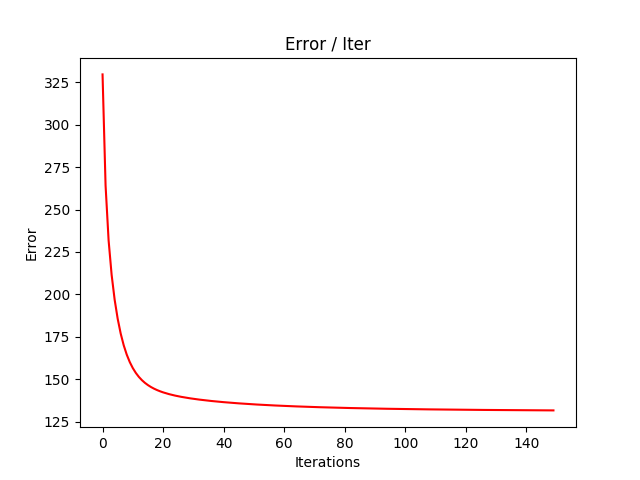
\includegraphics[width=0.5\textwidth]{images/err_dset2.png}

\break

\textbf{Distance function:}
The output of my code for distance function of dataset2

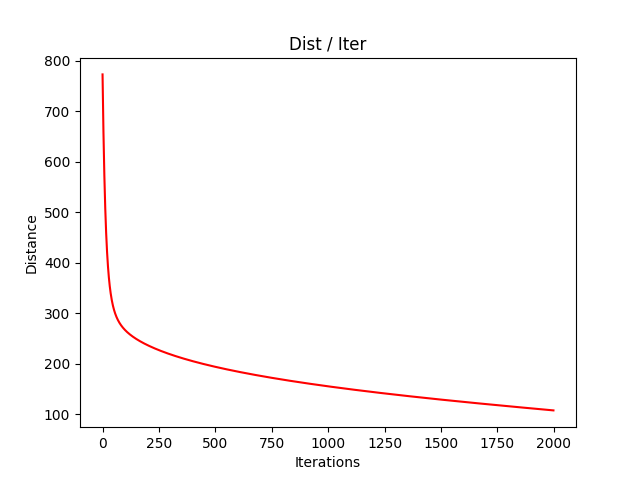
\includegraphics[width=0.5\textwidth]{images/dist_dset2.png}

\end{enumerate}

\end{document}
